\chapter{Einleitung}
\label{ch:Einleitung}
Während die Ortung im Außenbereich fest in der Hand von Satellitensystemen wie dem Global Positioning System (GPS) liegen, bietet die Ortung im Innenraum eine Vielzahl verschiedener Technologien. Neben Technologien wie Bluetooth, Radio Frequency Identification (RFID) und Ultra Wide Band (UWB) weckt WLAN wegen seiner großen Verbreitung immer wieder Interesse in Forschung und Industrie. \\
So hat die Ortung mittels WLAN gerade im medizinischen Bereich durch kommerzielle Lösungen Verbreitung gefunden, Probleme finden sich aber bei Ortungsgenauigkeit gegenüber anderen Techniken und dem vergleichsweise hohen Energieverbrauch des WLAN Protokolls.
Während sich viele wissenschaftliche Arbeiten der Ortungsgenauigkeit widmen, ist für den alltäglichen Einsatz die kurze Batterielaufzeit der mobilen Einheiten hinderlich, wenn nicht zum Beispiel Smartphones als mobile Einheiten in Frage kommen. \\
Auch im Tunnelbau ist eine Ortung von Mitarbeitern und Besuchern von Nöten um in Notfällen bestimmen zu können, ob und wie viele Personen sich im Gefahrenbereich befinden, dies beeinflusst die Arbeit der Rettungskräfte. 
Das veränderliche Umfeld der Baustelle, auf der große Stahl- und Betonelemente bewegt werden, stellt dabei die genaue Ortung mittels Radiowellen vor große Probleme und es wird nur eine Bereichsortung durchgeführt, bei der jede Tunnelröhre in mehrere hundert Meter große Abschnitte aufgeteilt wird und der Wechsel der Mitarbeiter zwischen den Abschnitten beobachtet wird. 
Dies stellt zwar nur eine geringe Genauigkeit dar, erlaubt es aber bei Bränden zu erkennen welche Personen sich durch die Abschnitte Richtung Ausgang bewegen und welche in ihrem Abschnitt verharren, sie sind vermutlich bewegungsunfähig oder eingeschlossen.\\ 


\section{Bisherige Situation}
Die Ortung wird derzeit bei der Ed. Züblin AG mittels Bluetooth durchgeführt, dabei sind die Basisstationen eigenständige Bluetooth-Einheiten die mit dem Ethernet Backbone verbunden sind.
Als mobile Einheiten kommen sowohl batteriebetriebene Tags als auch Smartphones zum Einsatz. 
Das zentrale Sicherheitssystem fragt die gesehenen mobilen Einheiten bei den Basisstationen an und bereitet die Ergebnisse graphisch auf.\\
Der Tunnel wird in Bereiche zu circa 500 Meter aufgeteilt, die Tunnelbohrmaschine (TBM) stellt dabei einen Sonderbereich dar, weil sie sich im Gegensatz zu den anderen Bereichen langsam bewegt. 
Neue Bereiche werden hinter der TBM eingefügt und sind dann stationär.\\
Die Bluetooth Basisstationen werden in Kästen verstaut die weitere notwendige Technik, wie etwa ein Notfalltelefon, enthalten.
Weil diese Kästen nur etwa alle 500 Meter montiert sind, existieren große Lücken in denen die mobilen Einheiten nicht geortet werden.
Eine mobile Einheit bleibt im System so lange in einem Bereich bis sie wieder von einer Basisstation erkannt wird.\\
Wird die mobile Einheit von der Erfassungseinheit vor dem Portal (Tunneleingang) erkannt gilt sie als außerhalb des Tunnels.
Abbildung \ref{fig:bisherige} zeigt die bisherige Situation mit Bluetooth Basissationen, die Reichweite der der Basistationen ist dabei nicht maßstabsgetreu.

\begin{figure}[h]
  \centering
	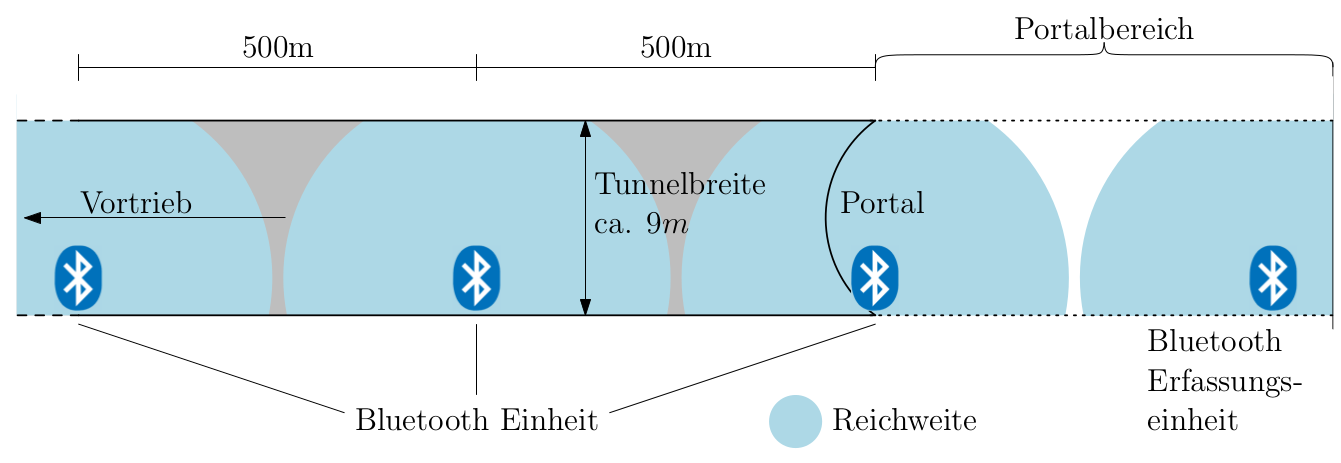
\includegraphics[width=\textwidth]{images/bisherige.png}
  \caption{Bereichsortung mit Bluetooth, aus \cite{maurer2016unterstuetzung}.}
  \label{fig:bisherige}
\end{figure}

 
\section{Umgebung für funkbasierte Ortung}
Als Versuchsumgebung dient die Tunnelbaustelle Rastatt.
Dort gelten die Positionen der Kästen für die Technik als unveränderlich.
Nur sie bieten Strom, Netzwerkanbindung (LAN) und Schutz vor dem Baustellenumfeld.
Für Funkprotokolle, die weniger als 250 Meter Reichweite haben muss daher mit Erfasssungslücken gerechnet werden.
Auf der TBM und anderen technischen Fahrzeugen sind jedoch mehr Basisstationen möglich.\\
Es existiert bereits ein WLAN Netzwerk, dessen Access Points als Basisstationen genutzt werden können.
Es handelt sich um APs der Firma Lancom, diese stellt auch einen LN-862 für Versuche.
Für zukünftige Baustellen soll der Abstand der Versorgungskästen auf 250 Meter sinken, diese Situation ist in Abbildung \ref{fig:zukuenftige} skizziert.

\begin{figure}[h]
  \centering
	\includegraphics[width=\textwidth]{images/zukuenftige.eps}
  \caption{Zukünftige Situation der Tunnelbaustellen.}
  \label{fig:zukuenftige}
\end{figure}

\section{Zielsetzung der Arbeit}
\label{ch:Einleitung:sec:Zielsetzung}
Ziel der Arbeit soll der Entwurf und die Implementierung eines Bereichsortungssystems für Personen in Tunnelanlagen unter Verwendung eines bestehenden Netzwerks von WLAN Access Points (APs) sein. 
Bei einem Bereichsortungssystem handelt es sich um ein Ortungssystem, bei dem die Positionen nicht genau bestimmt werden. 
Stattdessen wird das Areal, auf dem geortet werden soll, in einzelne Bereiche unterteilt und jede mobile Einheit beim Vorgang des Ortens einem dieser Bereiche zugeordnet.\\
Diese Arbeit grenzt sich von vorherigen Arbeiten dadurch ab, dass die Laufzeit beziehungsweise der Energieverbrauch der mobilen Einheiten im Vordergrund steht. 
Statt der nur wenige Tage umfassenden Laufzeiten anderer WLAN basierter Tags ist das Ziel dieser Arbeit eine Laufzeit von mehreren Monaten. \\
Der Entwurfsraum umfasst in einem ersten Schritt keine Änderungen an den Access Points, ihre Anzahl, Position, Software und Hardware ist gegeben. \\ %TODO Dev findet Satz doofi
Anschließend wird diese Beschränkung gelockert und die Software der APs kann verändert werden, bei diesen Veränderungen sollen aber die grundlegenden Mechanismen der 802.11 Spezifikation erhalten bleiben. 
So soll es nicht assozierten Clients nicht möglich sein direkt mit Servern im Netzwerk zu kommunizieren, da dies die Sicherheit des gesamten Netzwerks gefährden könnte.\\
In einer zweiten Lockerung der Beschränkungen soll auch die Hardware veränderbar sein, dies widerspricht zwar der Annahme der bestehenden Struktur von WLAN APs, da diese potenziell ausgetauscht werden müssten, erweitert den Handlungsspielraum jedoch enorm und erlaubt es die vorherigen Implementierungen mit einer energetisch effizienten und potenziell nicht WLAN-basierten Protokollen zu vergleichen. \\
Für jeden dieser Schritte müssen die angrenzenden Komponenten (Ortungsserver und mobile Einheiten) implementiert und hinsichtlich des Energieverbrauchs und der Erkennungssicherheit evaluiert werden. Abschließend sollen die drei Systeme miteinander verglichen werden. \\


\section{Anforderungen an das Bereichsortungssystem}
\label{ch:Einleitung:sec:Anforderungen}
Da es sich um ein Bereichsortungssystem handeln soll, werden keine direkten Anforderungen an die Genauigkeit der Ortung gestellt, jedoch soll ein klarer Wechsel zwischen zwei Bereichen, und damit zwei Basisstationen, zuverlässig erkannt werden. 
Bei den von den Zielpersonen getragenen Positionssendern, den mobilen Einheiten, soll es sich in den ersten beiden Schritten um Geräte handeln, die auf WLAN Basis arbeiten und somit mit den APs kompatibel sind.
Im dritten Schritt ist dies nicht erforderlich und die Kompatibilität wird durch technische Änderungen am AP wiederhergestellt.
Die Tags sollen eine Laufzeit von bis zu drei Jahren erreichen, sie sollen jedoch mindestens eine Laufzeit von sechs Monaten aufweisen, um als verwendbar angesehen zu werden. 
Dabei sind Größe und Gewicht der Lösung zu beachten, zwar kann die Laufzeit eines Tags jederzeit durch die Vergrößerung des Energiespeichers herbeigeführt werden, die Tags müssen jedoch mühelos von den Zielpersonen an einem Band um den Hals getragen werden können.
Zuletzt soll unter Rücksichtnahme auf das beschriebene Szenario die Komplexität der IT-Infrastruktur so gering wie möglich gehalten werden um ein stabiles und kostengünstiges System zu garantieren. 


\section{Gliederung der Arbeit}
\label{ch:Einleitung:sec:Gliederung}
Nachdem zunächst in Kapitel \ref{ch:Grundlagen} die Grundlagen der funkbasierten Ortung und der verwendeten Funkprotokolle behandelt werden, wird in Kapitel \ref{ch:Grundlagen} das Problem analysiert und verwandte Arbeiten aufgezeigt.
Die Kapitel \ref{ch:phase1}, \ref{ch:phase2} und \ref{ch:phase3} beschäftigen sich mit der Implementierung. 
Kapitel \ref{ch:phase1} behandelt die Ortung ohne Änderungen an den APs, Kapitel \ref{ch:phase2} erlaubt Änderungen der Software der APs und die Implementierung aus Kapitel \ref{ch:phase3} basiert nicht auf WLAN und erfordert daher zusätzliche Hardware.
In Kapitel \ref{ch:Beschleunigungssensor} wird die Integration eines Beschleunigungssensors zur Verlängerung der Laufzeit diskutiert.
Kapitel \ref{ch:Reichweite} beeinhaltet die Versuche bezüglich der Reichweite von WLAN und Bluetooth im Tunnel, anschließend werden in Kapitel \ref{ch:Vergleich} die Lösungen bezüglich ihres Energieverbrauchs verglichen.
Das Fazit in Kapitel \ref{ch:Fazit} fasst die Arbeit noch einmal zusammen, bewertet die Ergebnisse und beschließt die Arbeit.
